%% FullCourse_10Lecs -- Lecture 7, Act 3 (ATTEND, part 2/2): The Transformer
%% ch14 rebuild (2026-07-07), per Lec07_ch14_Rebuild_Plan_2026-07-07.md.
%% Reused frames copied verbatim (with renumbered cross-references) from
%%   archive_pre_split/pre_ch14_rebuild_2026-07-07/Lec07_T2b_Transformer_Architecture.tex (layer, variants, Kim case)
%%   archive_pre_split/pre_ch14_rebuild_2026-07-07/Lec07_T2a_Attention_Mechanism.tex (positional-encoding trio,
%%     output-embeddings-to-next-token, real LLM scale -- these lived in T2a, not T2b)
%% "Inside a Layer (Preview)" dropped (superseded by the full treatment here).
%% New frames follow chapter14 sec. 14.4.2-3: why-Transformer-beats-RNN techbox;
%% FFN frame enriched with the Geva 2021 key-value-memory reading.

%% Shared preamble for the FullCourse_10Lecs topic decks.
%%
%% Each topic .tex \input's this file, then defines its own \title, \date
%% override (if any), \graphicspath, and \begin{document}.
%%
%% Reconstructed verbatim from the inlined copy preserved in
%% Lec10_Case_Studies/Lec10_T8_Case6_DeepRamsey.tex (lines 23-190), which is
%% explicitly annotated there as "from ../shared_preamble.tex, copied verbatim".
%% Base preamble matches MiniCourse_8hr/Slides/shared_preamble.tex; this version
%% additionally provides \sectiondivider, the conceptbox/cautionbox/examplebox/
%% takeawaybox tcolorboxes, and \compacttables used across the split decks.

\documentclass[10pt,english,aspectratio=169]{beamer}

\usepackage{ae,aecompl}
\usepackage[T1]{fontenc}
\usepackage{textcomp}
\usepackage[utf8]{inputenc}
\usepackage{babel}
\usepackage{datetime2}

\setcounter{secnumdepth}{3}
\setcounter{tocdepth}{3}

\usepackage{amsmath, amssymb, amsthm, graphicx}
\usepackage{booktabs, multirow}
\usepackage{tikz}
\usepackage{pgfplots}
\pgfplotsset{compat=1.16}
\usepackage[most]{tcolorbox}
\tcbuselibrary{skins, breakable, theorems}
\usepackage{listings}
\usepackage{xcolor}

\lstset{
  basicstyle=\ttfamily\small,
  keywordstyle=\color{blue!80!black}\bfseries,
  commentstyle=\color{green!50!black}\itshape,
  stringstyle=\color{orange!80!black},
  backgroundcolor=\color{gray!8},
  frame=single,
  rulecolor=\color{gray!40},
  breaklines=true,
  showstringspaces=false,
  numbers=none,
}

\lstdefinestyle{pythonstyle}{
    language=Python,
    basicstyle=\ttfamily\footnotesize,
    keywordstyle=\color{blue!80!black}\bfseries,
    commentstyle=\color{green!50!black}\itshape,
    stringstyle=\color{orange!80!black},
    frame=single,
    breaklines=true,
    showstringspaces=false,
    numbers=left,
    numbersep=5pt,
    numberstyle=\tiny\color{gray},
    backgroundcolor=\color{gray!8},
    rulecolor=\color{gray!40}
}

\ifx\hypersetup\undefined
  \AtBeginDocument{%
    \hypersetup{bookmarks=false,breaklinks=true,pdfborder={0 0 0},colorlinks=true,
      linkcolor=DarkText,urlcolor=RedTitle}%
  }
\else
  \hypersetup{bookmarks=false,breaklinks=true,pdfborder={0 0 0},colorlinks=true,
    linkcolor=DarkText,urlcolor=RedTitle}%
\fi

\makeatletter
\newcommand\makebeamertitle{%
  \begin{frame}[plain]
    \vspace*{1.0cm}
    \centering
    {\usebeamerfont{title}\usebeamercolor[fg]{title}\inserttitle\par}
    \vspace{1.0cm}
    {\usebeamerfont{author}\usebeamercolor[fg]{author}\insertauthor\par}
    \vspace{0.2cm}
    {\usebeamerfont{date}\usebeamercolor[fg]{date}\insertdate\par}
  \end{frame}}%
\AtBeginDocument{%
  \let\origtableofcontents=\tableofcontents
  \def\tableofcontents{\@ifnextchar[{\origtableofcontents}{\gobbletableofcontents}}
  \def\gobbletableofcontents#1{\origtableofcontents}%
}

\usetheme{metropolis}
\usefonttheme{professionalfonts}

\definecolor{LightGray}{RGB}{230,230,230}
\definecolor{RedTitle}{RGB}{0,0,200}
\definecolor{VeryLightGray}{RGB}{245,245,245}
\definecolor{DarkText}{RGB}{0,0,0}

\setbeamercolor{background canvas}{bg=white}
\setbeamercolor{title}{fg=RedTitle}
\setbeamercolor{author}{fg=DarkText}
\setbeamercolor{date}{fg=DarkText}
\setbeamercolor{frametitle}{bg=VeryLightGray,fg=DarkText}
\setbeamercolor{normal text}{fg=DarkText}
\setbeamerfont{title}{size=\large}

\setbeamersize{text margin left=5mm, text margin right=5mm}
\addtobeamertemplate{frametitle}{}{\vspace{-0.5em}}
\newcommand{\reducevspace}{\vspace{-0.5cm}}

% Shared section divider and box styles for split topic decks.
\newcommand{\sectiondivider}[2]{%
\begin{frame}[plain,noframenumbering]
\begin{center}
\vfill
{\Large\textbf{#1}\par}
\vspace{0.35cm}
{\normalsize #2\par}
\vfill
\end{center}
\end{frame}
}

\newtcolorbox{conceptbox}[1][]{
  colback=blue!3,
  colframe=RedTitle!55,
  boxrule=0.35mm,
  arc=1mm,
  left=2mm,
  right=2mm,
  top=1mm,
  bottom=1mm,
  #1
}
\newtcolorbox{cautionbox}[1][]{
  colback=red!3,
  colframe=red!50!black,
  boxrule=0.35mm,
  arc=1mm,
  left=2mm,
  right=2mm,
  top=1mm,
  bottom=1mm,
  #1
}
\newtcolorbox{examplebox}[1][]{
  colback=green!3,
  colframe=green!45!black,
  boxrule=0.35mm,
  arc=1mm,
  left=2mm,
  right=2mm,
  top=1mm,
  bottom=1mm,
  #1
}
\newtcolorbox{takeawaybox}[1][]{
  colback=VeryLightGray,
  colframe=RedTitle!55,
  boxrule=0.35mm,
  arc=1mm,
  left=2mm,
  right=2mm,
  top=1mm,
  bottom=1mm,
  #1
}
\newcommand{\compacttables}{\renewcommand{\arraystretch}{1.15}}

\setbeamertemplate{navigation symbols}{}
\setbeamertemplate{footline}{%
  \hfill%
  \usebeamercolor[fg]{page number in head/foot}%
  \usebeamerfont{page number in head/foot}%
  \insertframenumber\,/\,\inserttotalframenumber\kern1em\vskip2pt%
}

\makeatother

\author{Zhigang Feng}
% "date with time": compile timestamp so each build is identifiable.
\date{\today\ \DTMcurrenttime}


\metroset{sectionpage=none}

\graphicspath{{./pic/}{../../MiniCourse_8hr/Slides/Module3_LLM_Text/pic/}{../}}

\usetikzlibrary{positioning,arrows.meta,shapes,calc,matrix,fit,backgrounds}

%% Lec07 shared MAP slide: "one map, five acts" recurring diagram.
%% Adapted from ../Lec09_Agentic_AI/lec09_map.tex (\LecNineMap -> \LecSevenMap).
%% Input this file AFTER ../shared_preamble.tex (needs RedTitle, VeryLightGray)
%% and call \LecSevenMap{k} inside a frame, where k in {1..5} highlights the
%% current act ("you are here") and k = 0 renders the closing reprise with all
%% five acts complete (used by T5b's closing frame).
%% Filename deliberately does not match the build glob Lec*_T*.tex, so the
%% build script never tries to compile it standalone.

\newcommand{\LecSevenMap}[1]{%
% Precompute per-box style selectors; TikZ option lists are comma-split before
% TeX conditionals run, so \ifnum must not sit inside a [...] options list.
\ifnum#1=0
  \tikzset{lecmapa/.style={lecmapdone}, lecmapb/.style={lecmapdone},
           lecmapc/.style={lecmapdone}, lecmapd/.style={lecmapdone},
           lecmape/.style={lecmapdone}}%
\else
  \tikzset{lecmapa/.style={}, lecmapb/.style={}, lecmapc/.style={},
           lecmapd/.style={}, lecmape/.style={}}%
  \ifnum#1=1 \tikzset{lecmapa/.style={lecmapcur}}\fi
  \ifnum#1=2 \tikzset{lecmapb/.style={lecmapcur}}\fi
  \ifnum#1=3 \tikzset{lecmapc/.style={lecmapcur}}\fi
  \ifnum#1=4 \tikzset{lecmapd/.style={lecmapcur}}\fi
  \ifnum#1=5 \tikzset{lecmape/.style={lecmapcur}}\fi
\fi
\begin{center}
\begin{tikzpicture}[
    act/.style={rectangle, rounded corners, draw=black!60, fill=VeryLightGray,
        minimum width=2.6cm, minimum height=0.92cm, text width=2.5cm,
        align=center, font=\scriptsize, text=DarkText},
    lecmapcur/.style={draw=RedTitle, very thick, fill=orange!20},
    lecmapdone/.style={draw=green!45!black, thick, fill=green!10},
    q/.style={font=\tiny\itshape, text width=2.7cm, align=center, text=black!70},
    sat/.style={rectangle, rounded corners, draw=black!45, dashed, fill=white,
        text width=5.0cm, align=center, font=\tiny, text=black!70,
        minimum height=0.5cm},
    barlab/.style={font=\tiny\bfseries, text=black!60},
    arr/.style={-{Stealth[length=2mm]}, thick, gray!60}
]
    % --- five act boxes ---
    \node[act, lecmapa] (a1) at (0,0)
        {\textbf{7.1 FRAME}\\ \tiny text as measurement};
    \node[act, lecmapb] (a2) at (2.85,0)
        {\textbf{7.2 REPRESENT}\\ \tiny tokens $\to$ vectors};
    \node[act, lecmapc] (a3) at (5.7,0)
        {\textbf{7.3 ATTEND}\\ \tiny attention \& Transformer};
    \node[act, lecmapd] (a4) at (8.55,0)
        {\textbf{7.4 PRETRAIN}\\ \tiny LMs \& alignment};
    \node[act, lecmape] (a5) at (11.4,0)
        {\textbf{7.5 MEASURE}\\ \tiny limits, apps, validation};
    \draw[arr] (a1) -- (a2);
    \draw[arr] (a2) -- (a3);
    \draw[arr] (a3) -- (a4);
    \draw[arr] (a4) -- (a5);
    % --- the student question each act answers ---
    \node[q] at (0,-0.82)    {what generates\\ this text?};
    \node[q] at (2.85,-0.82) {how do we turn it\\ into numbers?};
    \node[q] at (5.7,-0.82)  {how does context\\ get encoded?};
    \node[q] at (8.55,-0.82) {where does a pretrained\\ model come from?};
    \node[q] at (11.4,-0.82) {is my measure valid ---\\ and defensible?};
    % --- "you are here" marker above the current act ---
    \ifnum#1=1 \node[font=\scriptsize\bfseries, text=RedTitle] at (0,0.95)
        {you are here\ $\blacktriangledown$};\fi
    \ifnum#1=2 \node[font=\scriptsize\bfseries, text=RedTitle] at (2.85,0.95)
        {you are here\ $\blacktriangledown$};\fi
    \ifnum#1=3 \node[font=\scriptsize\bfseries, text=RedTitle] at (5.7,0.95)
        {you are here\ $\blacktriangledown$};\fi
    \ifnum#1=4 \node[font=\scriptsize\bfseries, text=RedTitle] at (8.55,0.95)
        {you are here\ $\blacktriangledown$};\fi
    \ifnum#1=5 \node[font=\scriptsize\bfseries, text=RedTitle] at (11.4,0.95)
        {you are here\ $\blacktriangledown$};\fi
    \ifnum#1=0 \node[font=\scriptsize\bfseries, text=green!45!black] at (5.7,0.95)
        {all five acts complete};\fi
    % --- bottom band: the measurement sandwich ---
    \fill[blue!10]   (-1.3,-1.55) rectangle (1.40,-1.22);
    \fill[green!10]  (1.65,-1.55) rectangle (9.85,-1.22);
    \fill[orange!15] (10.1,-1.55) rectangle (12.7,-1.22);
    \node[barlab] at (0.05,-1.385) {WHY TEXT = MEASUREMENT};
    \node[barlab] at (5.75,-1.385) {HOW THE MACHINE READS TEXT};
    \node[barlab] at (11.4,-1.385) {MEASURE, VALIDATE, DISCLOSE};
    % --- the recurring spine (text DGP), printed under the band ---
    \node[font=\tiny\itshape, text=black!60] at (5.7,-1.83)
        {the spine:\ \ $x_i = g(s_i,\,a_i,\,c_i)+\varepsilon_i
         \;\longrightarrow\; m(x_i)
         \;\longrightarrow\; y_i = \beta\,m(x_i)+\gamma z_i+u_i$};
    % --- dashed satellites: the neighbouring lectures ---
    \node[sat] at (2.0,-2.42)
        {\textit{before 7.1:} Lec03--04 gave you neural nets, backprop \& PyTorch --- Lec07 teaches them to read};
    \node[sat] at (9.8,-2.42)
        {\textit{after 7.5:} Lec08 RAG (grounded memory) $\to$ Lec09 agents (grounded action) $\to$ Lec10 cases};
\end{tikzpicture}
\end{center}
}


\title[AI for Econ Research]{AI for Economic Research: Dynamic Models, Language, and Agents\\
Lecture 7.3b: The Transformer}

\begin{document}

\makebeamertitle

%=============================================================================
\begin{frame}{Lecture 7 in One Map}
\LecSevenMap{3}
\medskip
\textit{\footnotesize Route: wrap the attention head into a full layer (part 2/2 of ATTEND) --- position, residual, FFN $\to$ stack $L$ layers $\to$ pick among three variants $\to$ read 77{,}000 10-Ks with the same machinery.}
\end{frame}

%=============================================================================
\section{Completing the Layer}
\sectiondivider{Completing the Layer}{Position, residual safety nets, and the network that stores the knowledge}

\begin{frame}{Positional Encodings: Why They Are Needed}
\begin{itemize}
\item \textbf{Problem:} self-attention is \emph{permutation-equivariant} in its inputs. The tokens $\{\text{\emph{The}}, \text{\emph{Fed}}, \text{\emph{raised}}, \text{\emph{rates}}\}$ give the same internal state whether we read ``\emph{The Fed raised rates}'' or the scrambled ``\emph{Rates raised the Fed}'' --- yet the economic meaning is opposite (agent and patient are reversed). We must inject position.

\medskip
\item \textbf{Solution:} add a position vector $p(i)$ to each token embedding before the first layer:
\[
   e^{(i)} \;=\; \mathcal{E}\bigl(t^{(i)}\bigr) \;+\; p(i).
\]

\medskip
\item Three families of position encodings dominate practice. The choice matters most for \emph{long contexts} and \emph{length extrapolation}.

\medskip
\item \textbf{Take-away:} a Transformer must be \emph{told} where each token is. The mechanism is simple but indispensable.
\end{itemize}
\end{frame}

\begin{frame}{Sinusoidal, Learned, and Rotary (RoPE)}
\begin{itemize}
\item \textbf{Sinusoidal} (Vaswani et al., 2017) --- fixed, no parameters:
\[
   \mathrm{PE}(pos, 2i) = \sin\!\bigl(pos\,/\,10000^{2i/d}\bigr), \quad
   \mathrm{PE}(pos, 2i{+}1) = \cos\!\bigl(pos\,/\,10000^{2i/d}\bigr).
\]
Multiple frequencies $\Rightarrow$ relative offsets become linear functions; theoretically extrapolates beyond training length.

\medskip
\item \textbf{Learned} (BERT, original GPT) --- positions $1, \ldots, n_{\max}$ each get a learnable vector. Simple; \emph{cannot} extrapolate past $n_{\max}$.

\medskip
\item \textbf{Rotary (RoPE)} --- modern default in LLaMA, GPT-NeoX, Qwen, Mistral, DeepSeek. Apply a position-dependent \emph{rotation matrix} to $Q$ and $K$:
\[
   \langle R_{\theta_{i}} Q_i,\, R_{\theta_{j}} K_j\rangle \;=\; f(Q_i, K_j,\; i - j).
\]
Position information is baked into attention scores and depends only on \emph{relative} offset $i{-}j$ --- excellent length extrapolation.

\medskip
\item \textbf{ALiBi} (a close cousin) adds a linear distance penalty directly to attention scores; very simple, strong long-context behavior.
\end{itemize}
\end{frame}

\begin{frame}{Position Encodings: Trade-Off Table}
\begin{center}
\renewcommand{\arraystretch}{1.25}
\begin{tabular}{l c c c c}
\toprule
\textbf{Scheme} & \textbf{Params} & \textbf{Where applied} & \textbf{Extrapolates?} & \textbf{Modern use} \\
\midrule
Sinusoidal       & 0       & input embedding & yes (in theory) & rare today \\
Learned absolute & $n_{\max}\!\cdot\! d$ & input embedding & no & BERT, early GPT \\
RoPE             & 0       & inside $Q$, $K$ & yes (with scaling) & LLaMA, Qwen, Mistral \\
ALiBi            & $H$     & attention scores & yes & some long-context models \\
\bottomrule
\end{tabular}
\end{center}

\medskip
\begin{itemize}
\item \textbf{Take-away:} a Transformer must be \emph{told} where each token is. Modern LLMs prefer \emph{relative} schemes (RoPE / ALiBi) because they handle 32k+ context windows gracefully.
\end{itemize}
\medskip
\begin{takeawaybox}
\textbf{For long-document economics} --- complete 10-Ks (50k+ tokens), IMF country reports, decade-scale central-bank corpora --- prefer RoPE/ALiBi-based models. A fixed learned-absolute model simply cannot read past its training length.
\end{takeawaybox}
\end{frame}

\begin{frame}{Residual Connection and Layer Normalization}
\begin{itemize}
\item After the attention output $\tilde{e}^{(i)}$, the layer combines it with the original input via a \emph{residual connection} and then a \emph{layer normalization}:
\[
   u^{(i)} \;=\; \mathrm{Norm}\bigl(e^{(i)} \;+\; \tilde{e}^{(i)}\bigr).
\]

\medskip
\item \textbf{Why residual?}
\begin{itemize}
    \item Preserves the original information --- attention can only \emph{add} to it, never destroy it
    \item Provides a clean gradient path back through dozens of layers (the trick that made deep networks trainable)
\end{itemize}

\medskip
\item \textbf{Why layer normalization?}
\begin{itemize}
    \item Normalizes activations across the feature dimension to mean $0$, variance $1$
    \item Adds learnable scale $\gamma$ and shift $\beta$
    \item Stabilizes optimization dynamics, especially for very deep stacks
\end{itemize}
\end{itemize}
\end{frame}

\begin{frame}{Feed-Forward Network (MLP)}
\begin{itemize}
\item \textbf{Division of labor inside a layer.} Attention mixes information \emph{across} tokens; the FFN then transforms \emph{each} token individually given what it just gathered. Attention $=$ the meeting room; FFN $=$ desk work after the meeting.

\medskip
\item \textbf{Why it exists.} Attention alone is a linear map of value vectors. The FFN supplies the \emph{non-linear} transformation that lets the network represent arbitrary functions of a token's contextualized embedding.

\medskip
\item After attention + residual + norm, each position is passed independently through a small feed-forward network:
\[
   f^{(i)} \;=\; W_{2}\,\sigma\bigl(W_{1}\,u^{(i)} + b_{1}\bigr) + b_{2}.
\]

\medskip
\item \textbf{Shape conventions:} $W_{1}\colon d \!\rightarrow\! 4d$ (expand), activation $\sigma$ (ReLU / GELU / SwiGLU), $W_{2}\colon 4d \!\rightarrow\! d$ (contract). The $4d$ expansion is where most of an LLM's parameters live.

\medskip
\item \textbf{A useful reading --- key--value memory} (Geva et al.\ 2021): rows of $W_1$ act as \emph{pattern detectors} (``keys'': a collocation, a topic, an entity type); the ReLU selects which patterns fired; the matching columns of $W_2$ write back the associated content (``values''). Roughly $2/3$ of a layer's parameters sit here ($8d^2$ vs.\ attention's $4d^2$): attention \emph{moves} information to the right position, the FFN \emph{interprets} it against stored knowledge. Delete the FFNs and the model keeps its attention patterns but forgets its facts.

\medskip
\item Followed by another residual connection and layer normalization:
\[
   e'^{(i)} \;=\; \mathrm{Norm}\bigl(u^{(i)} + f^{(i)}\bigr).
\]
\end{itemize}
\end{frame}

\begin{frame}{One Layer --- Putting It All Together}
\begin{itemize}
\item A single Transformer layer can be summarized by the flow:
\[
   e^{(i)} \;\xrightarrow{\;\text{Self-Attention}\;}\; \tilde{e}^{(i)}
   \;\xrightarrow{\;\text{Res+Norm}\;}\; u^{(i)}
   \;\xrightarrow{\;\text{MLP}\;}\; f^{(i)}
   \;\xrightarrow{\;\text{Res+Norm}\;}\; e'^{(i)}.
\]

\medskip
\item Operationally:
\[
   \begin{aligned}
       \tilde{e}^{(i)} &\;=\; W_{O}\,\sum_{j} \alpha_{j}^{(i)}\,V_{j}, \\[2pt]
       u^{(i)} &\;=\; \mathrm{Norm}\bigl(e^{(i)} + \tilde{e}^{(i)}\bigr), \\[2pt]
       f^{(i)} &\;=\; W_{2}\,\sigma(W_{1}\,u^{(i)} + b_{1}) + b_{2}, \\[2pt]
       e'^{(i)} &\;=\; \mathrm{Norm}\bigl(u^{(i)} + f^{(i)}\bigr).
   \end{aligned}
\]

\medskip
\item Same $(\mathbb{R}^d)^n$ shape in and out: a layer is a structured non-linear update --- which is exactly what lets us stack it.
\end{itemize}
\end{frame}

\begin{frame}{After the Transformer: Where We Are}
\begin{itemize}
\item \textbf{What went in:} a sequence of $n$ tokens, converted to embeddings $+$ positional codes, $[e^{(1)}, \ldots, e^{(n)}]$ with each $e^{(i)} \in \mathbb{R}^{d}$.

\medskip
\item \textbf{What comes out of the top layer:} $n$ \emph{contextualized} vectors $[e'^{(1)}, \ldots, e'^{(n)}]$, same shape, same dimension. Each $e'^{(i)}$ encodes, in its $d$ coordinates,
\begin{itemize}
    \item (a) the identity of token $t^{(i)}$,
    \item (b) its syntactic / semantic role in \emph{this} sequence,
    \item (c) what every other token contributed to its meaning (causally masked in GPT-style models).
\end{itemize}

\medskip
\item \textbf{What we have NOT yet done:} no token generated, no class assigned, no number returned. Contextualized embeddings are an \textbf{intermediate data structure}, not the final answer.

\medskip
\item \textbf{What comes next:} a small \emph{task head} on top --- a vocabulary projection (generation) or a class projection (classification) --- turns the embeddings into the output we want.
\end{itemize}
\end{frame}

\begin{frame}{Stacking $L$ Layers}
\begin{itemize}
\item The output of one layer becomes the input of the next:
\[
   \bigl[e^{(1)}, \ldots, e^{(n)}\bigr]_{\text{layer } \ell + 1}
   \;\;=\;\;
   \bigl[e'^{(1)}, \ldots, e'^{(n)}\bigr]_{\text{layer } \ell}.
\]

\medskip
\item After $L$ layers, each token's vector has accumulated context from the entire sequence (subject to causal masking, in the autoregressive case).

\medskip
\item \textbf{Different layers learn different things} (empirically):
\begin{itemize}
    \item Lower layers: surface syntax, local agreement, morphology
    \item Middle layers: phrase- and clause-level structure
    \item Upper layers: discourse, factual associations, task-relevant abstractions
\end{itemize}

\medskip
\item \textbf{What we do with the top layer (``task heads'').}
\begin{itemize}
    \item \textbf{Generation:} logits $= W_{\text{vocab}}\, e'^{(n)}$, then $P(\text{next}=w) = \mathrm{softmax}(\text{logits})_{w}$. Training loss: $\mathcal{L} = -\sum_{i} \log P(t^{(i+1)} \mid t^{(1:i)})$ --- the same cross-entropy that shaped every weight in the stack during pretraining.
    \item \textbf{Classification:} logits $= W_{\text{class}}\, e'^{([\text{CLS}])}$, then $P(\text{class}=c) = \mathrm{softmax}(\text{logits})_{c}$. Training loss: $\mathcal{L} = -\sum \log P(y_{\text{true}} \mid x)$ on a labeled set (fine-tuned encoders: BERT, CentralBankRoBERTa, $\ldots$).
\end{itemize}
\end{itemize}
\end{frame}

\begin{frame}{RNN vs.\ Transformer: One Hidden State vs.\ All-to-All}
\begin{columns}[T]
\column{0.5\textwidth}
\centering
\textbf{RNN / LSTM} --- recurrence\\[1.5mm]
\begin{tikzpicture}[
  every node/.style={font=\scriptsize},
  st/.style={draw, circle, minimum size=6.5mm, fill=blue!12},
  arr/.style={-{Latex[length=1.2mm]}}
]
\node[st] (h1) {$h_1$};
\node[st, right=5mm of h1] (h2) {$h_2$};
\node[st, right=5mm of h2] (h3) {$h_3$};
\node[st, right=5mm of h3] (h4) {$h_4$};
\draw[arr] (h1)--(h2); \draw[arr] (h2)--(h3); \draw[arr] (h3)--(h4);
\foreach \i in {1,2,3,4}{\node[font=\tiny, below=3mm of h\i] (x\i) {$x_\i$}; \draw[arr] (x\i)--(h\i);}
\draw[arr, red!70!black, dashed] (h1) to[out=55,in=125]
   node[above, font=\tiny, red!70!black]{must survive 3 steps} (h4);
\end{tikzpicture}\\[1.5mm]
{\footnotesize $h_t = f(h_{t-1}, x_t)$: read left to right; the \emph{entire} past is squeezed into one fixed-size state, and must be computed \emph{in order}.}

\column{0.5\textwidth}
\centering
\textbf{Transformer} --- self-attention\\[1.5mm]
\begin{tikzpicture}[
  every node/.style={font=\scriptsize},
  tok/.style={draw, circle, minimum size=6.5mm, fill=orange!15},
  arr/.style={-{Latex[length=1.2mm]}}
]
\node[tok] (e1) {$e_1$};
\node[tok, right=5mm of e1] (e2) {$e_2$};
\node[tok, right=5mm of e2, fill=orange!45] (e3) {$e_3$};
\node[tok, right=5mm of e3] (e4) {$e_4$};
\draw[arr, orange!75!black] (e1) to[out=-45,in=-135] (e3);
\draw[arr, orange!75!black] (e2) to[out=-40,in=-140] (e3);
\draw[arr, orange!75!black] (e4) to[out=-135,in=-45] (e3);
\node[font=\tiny, above=1mm of e3] {gathers from all, 1 hop};
\end{tikzpicture}\\[1.5mm]
{\footnotesize $\mathrm{softmax}(QK^{\top}\!/\sqrt{d})\,V$: each token reads \emph{every} token directly, and \emph{all positions} are computed at once --- no state passed through time.}
\end{columns}
\medskip
\begin{itemize}
\item \textbf{The one difference everything follows from:} an RNN carries information \emph{through time} in a single vector; a Transformer accesses \emph{all positions at once}.
\item Path from token $j$ to token $i$: \textbf{$|i-j|$ update steps} in an RNN (signal decays, gradients vanish) vs.\ \textbf{one hop} in attention --- Vaswani et al.\ (2017), Table 1.
\item \textbf{The price:} attention costs $O(n^2)$ in sequence length vs.\ the RNN's $O(n)$ --- the reason long-context tricks (RoPE/ALiBi) and state-space models (Mamba) exist.
\end{itemize}
\end{frame}

\begin{frame}{Why the Transformer Displaced the RNN}
\textbf{Two compounding advantages --- each with an economic hook.}
\begin{conceptbox}
\textbf{1. Fully parallel training.} An LSTM must compute step $t$ after step $t-1$: $n$ tokens means $n$ serial steps. Attention over the whole sequence is two matrix multiplications, $\mathrm{softmax}\bigl(QK^{\top}/\sqrt{k}\bigr)V$ --- computed for all positions at once on a GPU. This is the engineering fact behind ``pretraining on billions of tokens became possible after 2017'': BERT's $3.3\times 10^9$-token pretraining was simply not feasible in serial mode.
\end{conceptbox}
\smallskip
\begin{conceptbox}
\textbf{2. $O(1)$ paths for long-range dependencies.} In a recurrent net, position $j$'s influence on a distant position $i$ must survive $i-j$ intermediate states --- the signal decays. Attention connects any two positions \emph{directly}. Concretely: Fed and PBOC policy reports state economic conditions in part 1 and the policy orientation pages later --- reading the guidance \emph{against} the conditions requires exactly these long jumps.
\end{conceptbox}
\smallskip
\textit{\footnotesize Post-script: state-space models (e.g.\ Mamba, Gu \& Dao 2023) revive recurrence with linear cost in sequence length --- worth watching for full-filing work, at some cost in exact global attention.}
\end{frame}

\begin{frame}{From Output Embeddings to the Next Token}
\begin{itemize}
\item For autoregressive generation we focus on the \emph{last} output vector $e'^{(n)}$.

\medskip
\item Project it onto the vocabulary with a linear layer:
\[
   \text{logits} \;=\; W_{\text{vocab}}\, e'^{(n)} \;+\; b_{\text{vocab}}, \qquad W_{\text{vocab}} \in \mathbb{R}^{M \times d}.
\]

\medskip
\item Convert logits to probabilities with softmax:
\[
   P\bigl(t^{(n+1)} = w \mid t^{(1)}, \ldots, t^{(n)}\bigr) \;=\; \frac{\exp(\text{logits}_{w})}{\sum_{j} \exp(\text{logits}_{j})}.
\]

\medskip
\item \textbf{Sampling strategies:} greedy, top-$k$, top-$p$ (nucleus), temperature scaling. (Unpacked in T4.)

\medskip
\item Append the chosen token to the context and repeat. \textbf{That} is how an LLM ``generates text''.
\end{itemize}
\end{frame}

\begin{frame}{Real LLM Scale}
\begin{center}
\renewcommand{\arraystretch}{1.3}
\begin{tabular}{l c c c c}
\toprule
\textbf{Quantity} & \textbf{Symbol} & \textbf{GPT-2} & \textbf{GPT-3} & \textbf{Modern (2024--26)} \\
\midrule
Layers & $L$ & 12--48 & 96 & 60--120 \\
Hidden dim & $d$ & 768--1600 & 12288 & 4096--16384 \\
Context length & $n$ & 1024 & 2048 & $32{\rm k}$--$1{\rm M}$ \\
Vocabulary & $M$ & 50k & 50k & 50k--256k \\
Parameters & --- & 0.1--1.5B & 175B & 70B--$>$1T \\
\bottomrule
\end{tabular}
\end{center}

\medskip
\begin{itemize}
\item \textbf{Modern open-weight examples (2024--2026):} LLaMA-3 (8B, 70B, 405B), DeepSeek-V3 (671B MoE), Qwen-2.5, Mistral.
\item \textbf{Modern closed examples:} GPT-4/5, Claude 3/4, Gemini (sizes undisclosed).
\item All share the same basic architecture; differences are scale, training data, and tuning --- the subject of Act 4.
\end{itemize}
\end{frame}

\begin{frame}{Transformer vs.\ Word2Vec}
\begin{center}
\renewcommand{\arraystretch}{1.3}
\begin{tabular}{l l l}
\toprule
\textbf{Property} & \textbf{Word2Vec} & \textbf{Transformer} \\
\midrule
Representation & 1 static vector / word & contextual vector / token \\
Architecture & 2-layer Skip-gram / CBOW & multi-head attention + MLP, deep stack \\
Context scope & fixed local window ($\pm5$) & full sequence, every token sees every token \\
Position info & none & explicit positional encodings \\
After training & lookup table; model discarded & model \emph{is} the network used downstream \\
Typical size & $\sim10^{7}$ params (CPU OK) & $10^{8}$--$10^{12}$ params (GPU required) \\
Best for & similarity, feature inputs & generation, classification, QA, RAG \\
\bottomrule
\end{tabular}
\end{center}

\medskip
\textbf{The big shift:} from a frozen lookup table of meanings to a deep, dynamic model where meaning emerges from interaction with context.
\end{frame}

%=============================================================================
\section{Three Variants}
\sectiondivider{Three Variants}{Same block, three masking patterns --- and three research uses}

\begin{frame}{Three Variants of the Same Block}
\begin{itemize}
\item The Transformer block is generic. The \emph{masking pattern} and the \emph{stack arrangement} determine what kind of model you get.

\medskip
\item \textbf{Encoder-only (BERT, RoBERTa, FinBERT, CentralBankRoBERTa)}
\begin{itemize}
    \item Bidirectional attention --- every token sees every other.
    \item Pretrained with \emph{masked language modeling}: hide tokens, predict from both sides.
    \item Best for: classification, embedding extraction, similarity. \emph{Not} a generator.
\end{itemize}

\medskip
\item \textbf{Decoder-only (GPT, LLaMA, Claude, Qwen)}
\begin{itemize}
    \item Causal mask --- each position only attends to itself and the past.
    \item Pretrained with \emph{next-token prediction}; autoregressive at inference (Act 4).
    \item Best for: open-ended generation, in-context learning, chat. The dominant paradigm today.
\end{itemize}

\medskip
\item \textbf{Encoder--Decoder (T5, BART, original Vaswani 2017)}
\begin{itemize}
    \item Encoder reads source bidirectionally; decoder generates target with causal $+$ cross-attention to encoder.
    \item Best for: translation, summarization, \textbf{structured extraction} --- e.g.\ turning free-form FOMC or PBOC minutes into (date, action, magnitude, guidance) database rows at a fraction of hand-coding cost.
\end{itemize}
\end{itemize}
\end{frame}

\begin{frame}{Picking a Variant for Your Macro Project}
\begin{center}
\renewcommand{\arraystretch}{1.3}
\footnotesize
\begin{tabular}{l l l l}
\toprule
\textbf{Task} & \textbf{Pick} & \textbf{Why} & \textbf{Example model} \\
\midrule
Sentiment / hawk--dove score on FOMC text & encoder & need a fixed embedding & CentralBankRoBERTa \\
Topic / event classification              & encoder & supervised fine-tune  & FinBERT, RoBERTa \\
Document embeddings for similarity / RAG  & encoder & pooled $e'^{([\text{CLS}])}$ & SBERT, BGE, E5 \\
Summarize a 10-K / press release          & enc--dec & input $\neq$ output & T5, BART \\
Structured extraction (minutes $\to$ rows) & enc--dec & learned text-to-schema map & T5, BART \\
Generate a forecast narrative             & decoder & open-ended text      & GPT-4, Claude, LLaMA \\
Q\&A over central-bank corpora (RAG)      & decoder $+$ retriever & generative w/ context & Lecture 8 \\
\bottomrule
\end{tabular}
\end{center}

\medskip
\begin{itemize}
\item \textbf{Rule of thumb.} If the output is a label or a vector, use an encoder. If the output is text, use a decoder. If you need to map one sequence to another and they have different lengths and structure, use encoder--decoder.
\end{itemize}
\end{frame}

\begin{frame}{``Attention Is All You Need'' (Vaswani et al., 2017) --- the Architecture}
\centering
\begin{tikzpicture}[
  every node/.style={font=\scriptsize},
  blk/.style={draw, rounded corners=1pt, minimum width=24mm, minimum height=4.2mm, align=center},
  enc/.style={blk, fill=blue!12},
  dec/.style={blk, fill=orange!15},
  io/.style={blk, fill=green!12, minimum width=20mm},
  arr/.style={-{Latex[length=1.2mm]}}
]
% --- ENCODER stack (left)
\node[io] (esrc) {source tokens $+$ pos};
\node[enc, above=2mm of esrc] (e1) {Multi-Head Self-Attn};
\node[enc, above=1.5mm of e1] (e2) {Add \& Norm};
\node[enc, above=1.5mm of e2] (e3) {Feed-Forward};
\node[enc, above=1.5mm of e3] (e4) {Add \& Norm};
\node[above=2mm of e4, font=\scriptsize\itshape] (eN) {$\times N$};
\draw[arr] (esrc)--(e1); \draw[arr] (e1)--(e2);
\draw[arr] (e2)--(e3);   \draw[arr] (e3)--(e4);
\node[draw, dashed, fit=(e1)(e4), inner sep=1.5mm, label=left:{\scriptsize\textbf{Encoder}}] {};

% --- DECODER stack (right)
\node[io, right=42mm of esrc] (dsrc) {target (shifted) $+$ pos};
\node[dec, above=2mm of dsrc] (d1) {Masked Multi-Head Self-Attn};
\node[dec, above=1.5mm of d1] (d2) {Add \& Norm};
\node[dec, above=1.5mm of d2] (d3) {Cross-Attn (Q from dec, K,V from enc)};
\node[dec, above=1.5mm of d3] (d4) {Add \& Norm};
\node[dec, above=1.5mm of d4] (d5) {Feed-Forward};
\node[dec, above=1.5mm of d5] (d6) {Add \& Norm};
\node[above=2mm of d6, font=\scriptsize\itshape] (dN) {$\times N$};
\node[blk, fill=gray!15, above=2mm of dN] (lin) {Linear $\to$ softmax};
\node[io, above=2mm of lin] (dout) {next-token probs};
\draw[arr] (dsrc)--(d1); \draw[arr] (d1)--(d2);
\draw[arr] (d2)--(d3);   \draw[arr] (d3)--(d4);
\draw[arr] (d4)--(d5);   \draw[arr] (d5)--(d6);
\draw[arr] (d6)--(lin);  \draw[arr] (lin)--(dout);
\node[draw, dashed, fit=(d1)(d6), inner sep=1.5mm, label=right:{\scriptsize\textbf{Decoder}}] {};

% --- cross-attention link
\draw[arr, thick, blue!60!black] (e4.east) to[out=0,in=180] node[above, font=\tiny]{K, V} (d3.west);
\end{tikzpicture}\\[1mm]
{\footnotesize Same block, two arrangements. Decoder-only models drop the encoder and the cross-attention.}
\end{frame}

\begin{frame}{Token Embeddings vs.\ Document Embeddings (Bridge to Lec08)}
\begin{columns}[T]
\column{0.55\textwidth}
\footnotesize
\begin{itemize}
\item \textbf{What the Transformer gives us directly.} For an $n$-token passage, the top layer outputs $n$ contextualized vectors $e'^{(1)}, \ldots, e'^{(n)} \in \mathbb{R}^{d}$ --- \emph{one per token}.

\medskip
\item \textbf{To compare whole passages we need one vector per passage.} Standard pooling moves:
\begin{itemize}
    \item \textbf{Mean-pool}: $\bar e = \tfrac{1}{n}\sum_i e'^{(i)}$ --- simple, surprisingly robust.
    \item \textbf{\texttt{[CLS]}-pool} (BERT family): use $e'^{([\text{CLS}])}$, trained to summarize the passage.
    \item \textbf{Learned pooling head}: a small attention head over the token sequence, trained for the downstream objective.
\end{itemize}

\medskip
\item \textbf{Retrieval embedders} (Sentence-BERT, BGE, E5, voyage-3) take a pretrained transformer and fine-tune it with a \emph{contrastive loss} on (anchor, positive, negative) triples: pull related passages together, push unrelated ones apart. The geometry is \emph{learned for similarity}, not inherited from the next-token objective.

\medskip
\item \textbf{Lec08 needs one vector per chunk to do retrieval.} Same transformer machinery, different head and different training signal.
\end{itemize}

\column{0.42\textwidth}
\centering
\begin{tikzpicture}[
  every node/.style={font=\scriptsize},
  tok/.style={draw, rounded corners=0.7pt, minimum width=8mm, minimum height=4mm, fill=blue!10},
  pool/.style={draw, rounded corners=1pt, minimum width=22mm, minimum height=4.5mm, fill=orange!15},
  doc/.style={draw, rounded corners=1pt, minimum width=22mm, minimum height=4.5mm, fill=green!18},
  arr/.style={-{Latex[length=1.2mm]}}
]
\node[font=\scriptsize\itshape] (lbl1) at (0,0) {$n$ token vectors};
\node[tok, below=2mm of lbl1] (t1) {$e'^{(1)}$};
\node[tok, right=1mm of t1] (t2) {$e'^{(2)}$};
\node[tok, right=1mm of t2] (t3) {$\cdots$};
\node[tok, right=1mm of t3] (t4) {$e'^{(n)}$};

\node[pool, below=5mm of t2.south east, xshift=-2mm] (p) {pool / \texttt{[CLS]} / head};
\draw[arr] (t1.south) -- (p.north west);
\draw[arr] (t2.south) -- (p.north);
\draw[arr] (t3.south) -- (p.north);
\draw[arr] (t4.south) -- (p.north east);

\node[doc, below=5mm of p] (d) {1 doc vector $\in\mathbb{R}^{d}$};
\draw[arr] (p) -- (d);

\node[below=2mm of d, font=\scriptsize\itshape, align=center] {Lec08: ranks $\cos(\text{query}, \text{doc})$};
\end{tikzpicture}
\end{columns}
\end{frame}

%=============================================================================
\section{Case: Reading 10-Ks at Paragraph Level}
\sectiondivider{Case: Reading 10-Ks at Paragraph Level}{Kim, Muhn, Nikolaev \& Zhang (2024) --- every concept of this act, reused}

\begin{frame}{From Tokens to Paragraphs: A Research Question}
\begin{itemize}
\item \textbf{Question.} Which language inside a 10-K filing actually moves stock prices? Press releases, MD\&A, risk factors, governance disclosures --- which content do investors \emph{react} to?

\medskip
\item \textbf{Paper.} Kim, Muhn, Nikolaev, Zhang (Booth WP, Nov.\ 2024), \emph{Learning Fundamentals from Text}.

\medskip
\item \textbf{The move.} Same Q/K/V machinery from T3a --- but the unit of analysis is a \textbf{paragraph}, not a word token. A 10-K is a sequence of $\sim 400$ paragraphs; treat each one as a ``token'' and let attention learn which paragraphs matter for the market.

\medskip
\item \textbf{Why this beats the standard playbook:}
\begin{itemize}
    \item Prior text-in-finance work collapses a 10-K to one number: sentiment (Loughran--McDonald 2011), uncertainty (Hassan et al.\ 2019). Information loss is severe.
    \item Attention preserves \emph{paragraph-level} granularity \emph{and} learns relational importance directly from market reactions.
    \item Trained attention weights are inspectable --- you can read off which content the market focuses on.
\end{itemize}
\end{itemize}
\end{frame}

\begin{frame}{Architecture: Two Attention Layers + MLP Head}
\begin{columns}[T]
\column{0.50\textwidth}
\footnotesize
\textbf{Pipeline} (full universe of EDGAR 10-Ks, 1996--2023, $\sim$77K filings, $\sim$20.7M paragraphs):
\begin{enumerate}
\item Split filing $\to$ paragraphs $p_1, \ldots, p_n$ (cap $n{=}1000$).
\item $e_i = \text{OpenAI \texttt{text-embedding-3-large}}(p_i)$, then truncate to first 64 dims (Matryoshka, Kusupati et al.\ 2022).
\item Stack $X = [e_1; \ldots; e_n] \in \mathbb{R}^{n\times 64}$, add sinusoidal positional encoding.
\item \textbf{Layer 1} --- Vaswani self-attention with residual: $\mathrm{Attention}(X)\!\in\!\mathbb{R}^{n\times 64}$.
\item \textbf{Layer 2} --- learned softmax pool to a doc vector:
\[
   X^{*} = \mathrm{softmax}\!\Bigl(\tfrac{W^{\top}\mathrm{Attention}(X)^{\top}}{\sqrt{64}}\Bigr)\,\mathrm{Attention}(X)
\]
with $W\!\in\!\mathbb{R}^{64}$ learnable; $X^{*}\!\in\!\mathbb{R}^{64}$.
\item MLP $(64{\to}128{\to}64{\to}1)$, ReLU, sigmoid $\to P(r_{[-1,+30]} > 0)$.
\end{enumerate}

\column{0.48\textwidth}
\centering
\begin{tikzpicture}[
  node distance=2.5mm,
  every node/.style={font=\scriptsize},
  box/.style={draw, rounded corners=1pt, minimum width=36mm, minimum height=4.4mm, align=center},
  io/.style={box, fill=green!12},
  emb/.style={box, fill=gray!18},
  attn/.style={box, fill=blue!12},
  pool/.style={box, fill=orange!18},
  mlp/.style={box, fill=red!12},
  arr/.style={-{Latex[length=1.4mm]}}
]
\node[io] (in) {10-K filing};
\node[emb, below=of in] (sp) {Split into paragraphs $p_i$};
\node[emb, below=of sp] (em) {OpenAI embed (3072$\to$64)};
\node[emb, below=of em] (pe) {$+$ sinusoidal pos.\ encoding};
\node[attn, below=of pe] (a1) {\textbf{Layer 1}: self-attention $+$ res.};
\node[pool, below=of a1] (a2) {\textbf{Layer 2}: softmax pool $\to X^{*}$};
\node[mlp, below=of a2] (mp) {MLP (128, 64, 1) $+$ ReLU};
\node[io, below=of mp] (out) {$P(r > 0)$};
\draw[arr] (in)--(sp);  \draw[arr] (sp)--(em);
\draw[arr] (em)--(pe);  \draw[arr] (pe)--(a1);
\draw[arr] (a1)--(a2);  \draw[arr] (a2)--(mp);
\draw[arr] (mp)--(out);
\end{tikzpicture}\\[2pt]
{\tiny Target: $\mathbb{1}\{r_{[\text{file}-1,\text{file}+30]} > 0\}$. Rolling 6/2/1-yr train/val/test.}
\end{columns}
\end{frame}

\begin{frame}{Every Concept from This Act, Reused}
\centering
\renewcommand{\arraystretch}{1.25}
\footnotesize
\begin{tabular}{l l}
\toprule
\textbf{Slide concept (this act)} & \textbf{Paper usage} \\
\midrule
$Q, K, V$ projections (T3a)                  & Same, but over \emph{paragraphs} not tokens \\
Scaled softmax $\mathrm{softmax}(QK^{\top}/\sqrt{d})V$ (T3a) & Used verbatim in Layer 1 \\
Sinusoidal positional encoding (T3b)         & Same Vaswani formula, scaled by embedding norm \\
Residual connection (T3b)                    & Added to Layer 1 output (paper fn.\ 13) \\
Cosine similarity (T2b)                      & Importance score: $\mathrm{cos}(e_i,\, X^{*})$ \\
Encoder-style training                       & \textbf{Supervised on returns}, not next-token \\
\bottomrule
\end{tabular}

\medskip
\begin{itemize}
\item \textbf{Methodological pivot.} A standard LLM trains attention with an unsupervised objective (next-token cross-entropy). This paper trains the \emph{same} attention machinery against a \textbf{financial target} (binary positive return). The attention weights then read directly as economic importance.

\medskip
\item \textbf{Importance score for paragraph $i$ in document $t$:}
\[
   \boxed{\;\;\text{Importance}_{ikt} \;=\; \frac{X_{it}^{*} \cdot e_{ikt}}{\|X_{it}^{*}\|\,\|e_{ikt}\|}\;\;}
\]
A paragraph is important when its semantic content aligns with the document's attention-weighted representation.
\end{itemize}
\end{frame}

\begin{frame}{Empirical Findings}
\begin{columns}[T]
\column{0.48\textwidth}
\footnotesize
\textbf{Predictive performance} (avg AUC, 20 yearly test sets, baseline $0.50$):
\begin{center}
\begin{tabular}{l c c}
\toprule
Model & AUC & $\Delta$ vs base \\
\midrule
Attention (paper) & \textbf{0.5599} & $+6.0$ pp \\
MLP (no attn)     & 0.5328 & $+3.3$ pp \\
Logit             & 0.5197 & $+2.0$ pp \\
\bottomrule
\end{tabular}
\end{center}

\smallskip
Sharpe (1-month-ahead returns): \textbf{1.56} attention, 1.28 MLP, 1.08 logit.

\medskip
\textbf{Attention share by 10-K Item} (stylized; learned weights):
\begin{center}
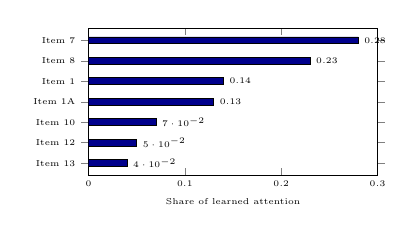
\begin{tikzpicture}[scale=0.62]
\begin{axis}[
  width=7.5cm, height=4.6cm,
  xbar,
  bar width=4pt,
  xmin=0, xmax=0.30,
  symbolic y coords={I13,I12,I10,I1A,I1,I8,I7},
  ytick=data,
  yticklabels={Item 13,Item 12,Item 10,Item 1A,Item 1,Item 8,Item 7},
  xlabel={Share of learned attention},
  tick label style={font=\tiny},
  label style={font=\tiny},
  nodes near coords,
  nodes near coords style={font=\tiny},
]
\addplot[fill=blue!55!black] coordinates {
  (0.04,I13)
  (0.05,I12)
  (0.07,I10)
  (0.13,I1A)
  (0.14,I1)
  (0.23,I8)
  (0.28,I7)
};
\end{axis}
\end{tikzpicture}\\
{\scriptsize Top: Item 7 MD\&A, Item 8 Financials. Bottom: Item 13 Relations, Item 12 Ownership, Item 10 Governance.}
\end{center}

\column{0.50\textwidth}
\footnotesize
\textbf{Topics inside MD\&A (Item 7):}
\begin{itemize}
\item \emph{Most attended}: segment information, financial performance, liquidity, recent M\&A.
\item \emph{Least attended}: forward-looking statements, accounting pronouncements, \textbf{corporate governance}, \textbf{sustainability / CSR}.
\end{itemize}

\smallskip
\begin{tcolorbox}[colback=LightGray, colframe=RedTitle, boxrule=0.3mm, arc=1mm, left=2mm, right=2mm, top=0.8mm, bottom=0.8mm]
\textbf{Surprise.} ESG and corporate governance --- dominant in public discourse --- rank \emph{lowest} by market reaction.
\end{tcolorbox}

\smallskip
\textbf{Two causal results.}
\begin{itemize}
\item SEC \emph{Modernization of Reg S-K} (treatment) raised Item 7 vs Item 8 (control) importance --- regulation can \emph{enhance} relevance.
\item Firms strategically place bad-news / low-profitability content \textbf{later} in MD\&A (Bloomfield 2008; Cohen et al.\ 2020) --- the DGP's $a_i$, visible in document structure.
\end{itemize}
\end{columns}
\end{frame}

%=============================================================================
\begin{frame}{Bridge: The Architecture Is Fixed --- Capability Is Not}
\textbf{Same block everywhere; the leverage now moves to training.}
\begin{itemize}
\item Kim et al.\ shows the pattern travels: change the ``token'' (paragraphs of a filing, sentences of a speech, stocks in a portfolio --- cf.\ Gabaix--Koijen--Richmond--Yogo's asset embeddings) and supervise attention on an economic target --- the weights become an inspectable measure.
\item But nothing so far explains where a model that already \emph{reads} comes from. GPT-2 to GPT-4 is essentially the same architecture --- what changed is pretraining scale, data, and alignment.
\item \textbf{Act 4:} self-supervised pretraining, prompting / fine-tuning / LoRA, and the SFT $+$ RLHF pipeline that turns a text-completer into an assistant --- plus what alignment does to measurement.
\end{itemize}
\bigskip
\centering\footnotesize\textit{Arc: T1 FRAME $\to$ T2 REPRESENT $\to$ \textbf{T3 ATTEND} $\to$ T4 PRETRAIN $\to$ T5 MEASURE.}
\end{frame}

\end{document}
